\subsection[Degradation network (1D)]{1D reactive transport: degradation of organic contaminants in a
sand column experiment by five bacterial groups forming a degradation network}
\label{l_s_benchmark_1d_network}

%Column experiments are often used to study the degradation of organic
%contaminants in the saturated groundwater zone.

The Biogeochemical Reaction Network
Simulator~(BRNS,~\cite{Aguilera2005,Regnier2002}) is coupled to GeoSys
following a sequential non-iterative operator splitting scheme yielding the
reactive transport model GeoSysBRNS. The technical
coupling is sketched in Fig.~\ref{fig:GeoSysBRNSSetup}.

\begin{figure}[h!]
\centering
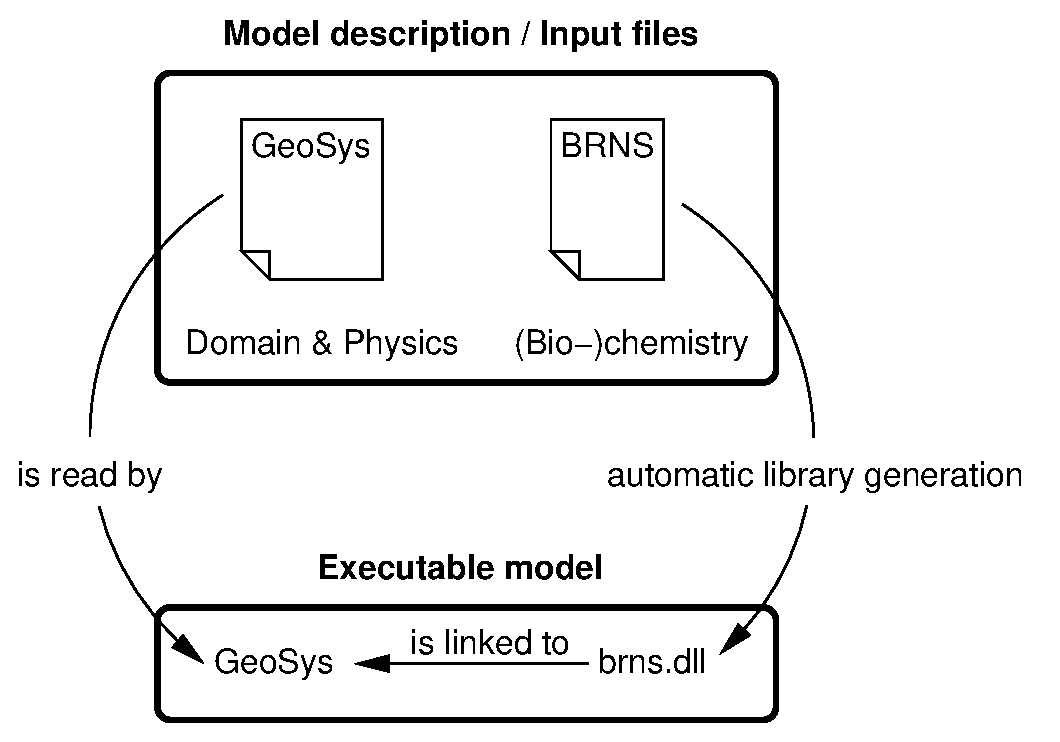
\epsfig{file=C/figures/GeoSysBRNSSetup.eps,width=8cm}
\caption{
The setup of GeoSysBRNS. The model description is divided into two parts: the
model domain definition, physical parameters, hydrogeological flow, and
discretization parameters in GeoSys format, and the description of the coupled
(bio-)chemical reaction processes in BRNS format. The latter is compiled into a
problem specific library that is accessed by GeoSys at runtime.
}
\label{fig:GeoSysBRNSSetup}
\end{figure}

\subsubsection*{The Model}

An experimental study by~\cite{Gunten1993} has been used to validate the
reactive transport models TBC~\cite{Schaefer1998b} and the stand-alone 1D
version of BRNS~\cite{Thullner2005}.  Both models could reproduce the
experimental data set. Here, we use the same simulation scenario to validate
GeoSysBRNS and compare simulation results to BRNS results.

In the example referred to as ``Scenario 1'' in~\cite{Thullner2005}, a sand
column of 29 centimeters length is constantly flushed with water containing
lactate as electron donor, and oxygen, nitrate, and sulfate as terminal
electron acceptors~(TEAs). Manganese and iron oxyhydroxides are bound to the
sand matrix in solid phases and act as two additional TEAs. Five distinct
microbial groups, which catalyze the reduction of each TEA to sustain their
growth, are considered in the model. The experimental results suggest that
lactate is concomitantly mineralized into dissolved inorganic carbon~(DIC) and
fermented to acetate and proprionate, with the latter being further oxidized
into DIC.  In addition to these microbial degradation pathways, reactive
species concentrations are influenced by a set of abiotic
reactions~(Fig.~\ref{fig:sandnetwork}).  The complete reaction network of the
model consists of 21 mobile and 18 immobile reactive species. The dynamics of
the system is determined by 24 kinetically controlled chemical reactions and
nine equilibrium reactions describing acid base dissociations.

\begin{figure}[h!]
$\bullet$ phase exchange (matrix, biophase, pore water)\\
$\bullet$ oxidation of sulfide by Fe(III)\\
$\bullet$ precipitation and dissolution of calcite and\\
Fe(II) minerals\\
$\bullet$ acid-base reactions for carbonates, sulfides,\\
lactate, propionate, acetate

\vspace{-2.75cm}
\hspace{8cm}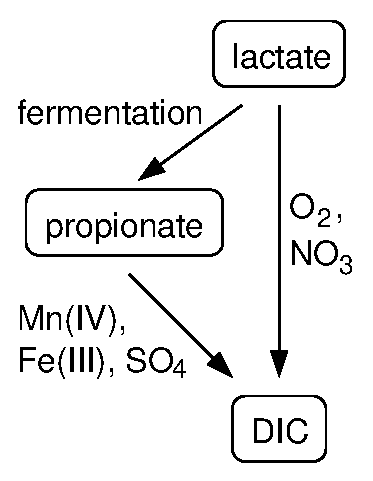
\epsfig{file=C/figures/GeoSysBRNSSandNetwork.eps,width=3.0cm}
\caption{
Modeling organic carbon degradation in a sand column experiment.  Coupled
abiotic processes considered in the model~(left), and microbial degradation
pathways with corresponding TAEs~(right).
}
\label{fig:sandnetwork}
\end{figure}

\subsubsection*{Evaluation method}

The coupling of the BRNS to GeoSys is shown to be correct by comparing
simulation results of GeoSysBRNS to BRNS results~\cite{Centler2009}.

\subsubsection*{Results}

We simulate the experiment with GeoSysBRNS using two spatial resolutions and
three different temporal resolutions per spatial setting, ensuring Courant
numbers smaller than 1.0 in all cases.  As in previous
studies~\cite{Thullner2005,Schaefer1998b}, we choose 48 days as the target
time for comparing the results of the coupled model to those obtained with the
BRNS model using the same set of spatio-temporal resolution settings.  At this
target time, the system is still in the transient phase. 

The simulation results of GeoSysBRNS and BRNS agree very well for all 39
reactive species at the highest spatial and temporal resolution~(see selected
species in Figs.~\ref{fig:columnresultsfine1},~\ref{fig:columnresultsfine2}).
Decreasing the spatial resolution leads to slightly different results, with the
coupled model generally staying closer to the high resolution result than the
stand-alone version of
BRNS~(Figs.~\ref{fig:columnresultsfine1},~\ref{fig:columnresultsfine2}).

When the time step size is increased, the numerical results of both models
diverge from the high resolution result~(Fig.~\ref{fig:columnresults}).  While
increasing the time step from 4 s to 43.2 s does not lead to significant
changes for both models and both spatial resolutions, a noticable deviation is
observed when the time step size is further increased to 108 s for the high,
and to 216 s for the low spatial resolution.  For these larger time step sizes,
the results of GeoSysBRNS are again generally closer to the high resolution
result than the BRNS solutions.  The observed differences can be attributed to
the different numerical schemes used by BRNS~(finite differences) and
GeoSysBRNS~(finite elements). Further details of the GeoSysBRNS and its
performance can be found in~\cite{Centler2009}.


\begin{table}[h!]
\centering
\begin{tabular}{|l|l|l|}
\hline
Benchmark & Type & Path \\
\hline
\texttt{1d\_degradation\_network}& C & benchmarks$\backslash$C$\backslash$1d\_degradation\_network \\
\hline
\end{tabular}
\end{table}

\begin{figure}[h!]
\centering
\epsfig{file=C/figures/GeoSysBRNSfinest_la_pro_ac.eps,angle=270,width=11cm}\\
\epsfig{file=C/figures/GeoSysBRNSfinest_biomass.eps,angle=270,width=11cm}
\caption{
Comparison of simulation results obtained with BRNS~(lines) and
GeoSysBRNS~(symbols): organic species~(top) and all five bacterial
groups~(bottom) at day 48 using the highest temporal resolution~($\Delta$t=4 s)
and two spatial resolutions. 
}
\label{fig:columnresultsfine1}
\end{figure}

\begin{figure}[h!]
\centering
\epsfig{file=C/figures/GeoSysBRNSfinest_nit_sul_mn.eps,angle=270,width=11cm}\\
\epsfig{file=C/figures/GeoSysBRNSfinest_s_fe.eps,angle=270,width=11cm}
\caption{
Comparison of simulation results obtained with BRNS~(lines) and
GeoSysBRNS~(symbols): inorganic species at day 48 using the highest temporal
resolution~($\Delta$t=4 s) and two spatial resolutions. 
}
\label{fig:columnresultsfine2}
\end{figure}

\begin{figure}[h!]
\centering
\epsfig{file=C/figures/GeoSysBRNSla_pro_ac.eps,angle=270,width=11cm}\\
\epsfig{file=C/figures/GeoSysBRNSla_pro_ac_fine.eps,angle=270,width=11cm}
\caption{
Comparison of simulation results obtained with BRNS~(lines) and
GeoSysBRNS~(symbols) at day 48 using two spatial resolutions~(top:
$\Delta$x=3.9mm, bottom: $\Delta$x=1.45mm) and different time step sizes for
lactate, proprionate, and acetate.
}
\label{fig:columnresults}
\end{figure}

\clearpage
